\documentclass[a4paper]{article}

\usepackage{tikz}

\newcommand{\pitch}{
  % The pitch
  \draw (0,0) rectangle (10.5,6.9);
  % Corner markers
  \filldraw [red] (0,0) circle (2pt)
                  (0,6.9) circle (2pt)
                  (10.5,0) circle (2pt)
                  (10.5,6.9) circle (2pt);
  % Half way lines
  \filldraw [red] (5.25,0) circle (2pt)
                  (5.25,6.9) circle (2pt);
  % 6 metre markers
  \filldraw [red] (1.8,0) circle (2pt)
                  (1.8,6.9) circle (2pt)
                  (8.7,0) circle (2pt)
                  (8.7,6.9) circle (2pt);
  % The goals
  %\filldraw (0,3.225) rectangle (-0.1,3.655);
  %\filldraw (10.5,3.225) rectangle (10.6,3.655);
}
\begin{document}
\begin{figure}
  \begin{tikzpicture}
    \pitch

    % One team set up in zone formation
    % Goalkeeper
    \filldraw [fill=green!20,draw=green!50!black] (0.15,3.45) ellipse (0.45 and 0.1);
    % Middle zone
    \filldraw [fill=green!20,draw=green!50!black] (1.3,3.45) ellipse (0.45 and 0.1);
    % Right zone
    \filldraw [fill=green!20,draw=green!50!black,rotate around={25:(1.2,2.45)}] (1.2,2.45) ellipse (0.45 and 0.1);
    % Left zone
    \filldraw [fill=green!20,draw=green!50!black,rotate around={155:(1.2,4.45)}] (1.2,4.45) ellipse (0.45 and 0.1);
    % Front of zone
    \filldraw [fill=green!20,draw=green!50!black,rotate around={80:(2.2,3.45)}] (2.2,3.45) ellipse (0.45 and 0.1);
  \end{tikzpicture}
  \caption{A basic 3 and 1 zone defence}
\end{figure}

\begin{figure}
  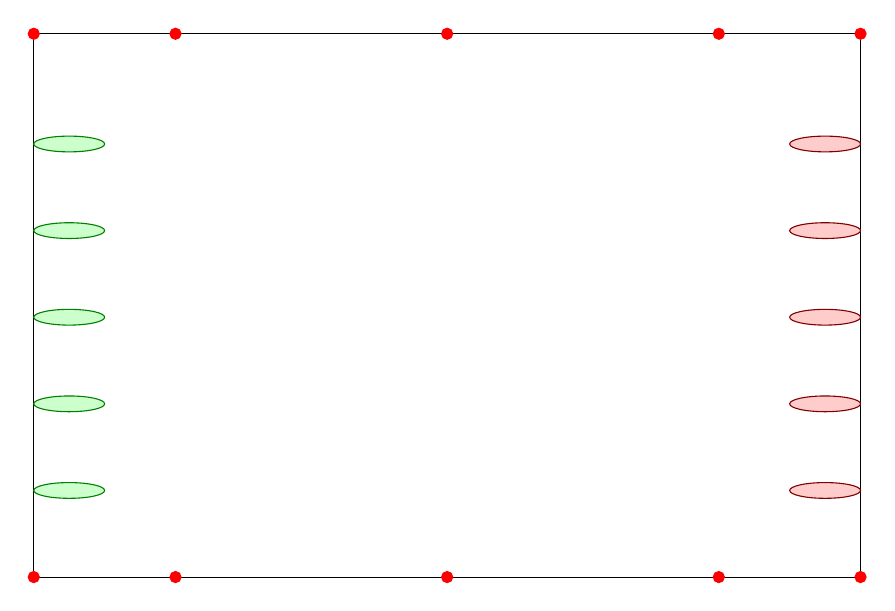
\begin{tikzpicture}
    \pitch

    % One team on the goal line
    \filldraw [fill=green!20,draw=green!50!black] (0.45,1.1) ellipse (0.45 and 0.1);
    \filldraw [fill=green!20,draw=green!50!black] (0.45,2.2) ellipse (0.45 and 0.1);
    \filldraw [fill=green!20,draw=green!50!black] (0.45,3.3) ellipse (0.45 and 0.1);
    \filldraw [fill=green!20,draw=green!50!black] (0.45,4.4) ellipse (0.45 and 0.1);
    \filldraw [fill=green!20,draw=green!50!black] (0.45,5.5) ellipse (0.45 and 0.1);

    % Other team on the goal line
    \filldraw [fill=red!20,draw=red!50!black] (10.05,1.1) ellipse (0.45 and 0.1);
    \filldraw [fill=red!20,draw=red!50!black] (10.05,2.2) ellipse (0.45 and 0.1);
    \filldraw [fill=red!20,draw=red!50!black] (10.05,3.3) ellipse (0.45 and 0.1);
    \filldraw [fill=red!20,draw=red!50!black] (10.05,4.4) ellipse (0.45 and 0.1);
    \filldraw [fill=red!20,draw=red!50!black] (10.05,5.5) ellipse (0.45 and 0.1);
  \end{tikzpicture}
  \caption{Lining up for the start of a half}
\end{figure}
\end{document}
